\RequirePackage{snapshot}
%%%%%%%%%%%%%%%%%%%%%%%%%%%%%%%%%%%%%%%%%%%%%%%%%%
% Basic setup. Most papers should leave these options alone.
\documentclass[fleqn,usenatbib]{mnras}

% MNRAS is set in Times font. If you don't have this installed (most LaTeX
% installations will be fine) or prefer the old Computer Modern fonts, comment
% out the following line
\usepackage{newtxtext,newtxmath}
% Depending on your LaTeX fonts installation, you might get better results with one of these:
%\usepackage{mathptmx}
%\usepackage{txfonts}

% Use vector fonts, so it zooms properly in on-screen viewing software
% Don't change these lines unless you know what you are doing
\usepackage[T1]{fontenc}

% Allow "Thomas van Noord" and "Simon de Laguarde" and alike to be sorted by "N" and "L" etc. in the bibliography.
% Write the name in the bibliography as "\VAN{Noord}{Van}{van} Noord, Thomas"
\DeclareRobustCommand{\VAN}[3]{#2}
\let\VANthebibliography\thebibliography
\def\thebibliography{\DeclareRobustCommand{\VAN}[3]{##3}\VANthebibliography}


%%%%% AUTHORS - PLACE YOUR OWN PACKAGES HERE %%%%%

% Only include extra packages if you really need them. Common packages are:
\usepackage{graphicx}	% Including figure files
\usepackage{amsmath}	% Advanced maths commands
\usepackage{fontawesome}
\usepackage[export]{adjustbox}

%%%%%%%%%%%%%%%%%%%%%%%%%%%%%%%%%%%%%%%%%%%%%%%%%%

%%%%% AUTHORS - PLACE YOUR OWN COMMANDS HERE %%%%%

\newcommand{\Msun}{M$_{\odot}$} % Msun (solar mass)
\newcommand{\microgauss}{$\mu$G} % microgauss
\newcommand{\vc}[1]{{\mathbf{#1}}}

% Workaround to fix the bug that prevents autoref from handling appendices properly
\newcommand{\aref}[1]{\hyperref[#1]{Appendix~\ref{#1}}}

% Autoref section names
\def\sectionautorefname{Section}
\def\subsectionautorefname{Section}
\def\subsubsectionautorefname{Section}
\def\paragraphautorefname{Section}
\def\figureautorefname{Figure}
\def\tableautorefname{Table}
\def\equationautorefname{equation}
\def\appendixautorefname{Appendix}

% Citation alias
\defcitealias{Colella_1984}{CW84}

% MRK's editing macros
\usepackage{color}
\usepackage[normalem]{ulem}
\definecolor{darkgreen}{rgb}{0.13, 0.55, 0.13}
\newcommand{\red}[1]{{\textcolor{red}{#1}}}
\newcommand{\cyan}[1]{{\textcolor{cyan}{#1}}}
\newcommand{\mrkcut}[1]{{\red{\sout{#1}}}}
\newcommand{\mrkadd}[1]{{\cyan{#1}}}
\newcommand{\mrknote}[1]{{\textcolor{darkgreen}{[MRK: #1]}}}

%%%%%%%%%%%%%%%%%%%%%%%%%%%%%%%%%%%%%%%%%%%%%%%%%%

%%%%%%%%%%%%%%%%%%% TITLE PAGE %%%%%%%%%%%%%%%%%%%

% Title of the paper, and the short title which is used in the headers.
% Keep the title short and informative.
\title[Two-moment AMR radiation hydrodynamics on GPUs]{\textsc{Quokka}: A new code for two-moment AMR radiation hydrodynamics on GPUs}

% The list of authors, and the short list which is used in the headers.
% If you need two or more lines of authors, add an extra line using \newauthor
\author[B. D. Wibking et al.]{
    Benjamin D. Wibking$^{1}$\thanks{E-mail: ben.wibking@anu.edu.au (BDW)}
    and Mark R. Krumholz$^{1}$
\\
% List of institutions
$^{1}$Research School of Astronomy \& Astrophysics, Mount Stromlo Observatory, Cotter Road, Weston Creek, ACT 2611 Australia\\
}

% These dates will be filled out by the publisher
\date{Accepted XXX. Received YYY; in original form ZZZ}

% Enter the current year, for the copyright statements etc.
\pubyear{2021}

% Don't change these lines
\begin{document}
\label{firstpage}
\pagerange{\pageref{firstpage}--\pageref{lastpage}}
\maketitle

% Abstract of the paper
\begin{abstract}
    We present a new subcycling-in-time, block-structured adaptive mesh refinement (AMR) radiation hydrodynamics code for graphics processing units (GPUs). The equations of hydrodynamics are solved with the piecewise parabolic method (PPM) in a method-of-lines formulation and the radiative transfer is solved via the variable Eddington tensor (VET) radiation moment equations with a local closure. We combine explicit-in-time evolution of the radiation moment equations with the reduced speed-of-light approximation. We show results for a wide range of test problems for hydrodynamics, radiation, and coupled radiation hydrodynamics. On uniform grids in 3D, we achieve a peak of $69$ million hydrodynamic updates per second per GPU. For radiation hydrodynamics problems on uniform grids in 3D, our code scales from 4 GPUs to 256 GPUs with an efficiency of $>93$ per cent. The code is publicly released under an open-source license on \faGithub\href{https://github.com/BenWibking/quokka-code}{GitHub}.
\end{abstract}

% Select between one and six entries from the list of approved keywords.
% Don't make up new ones.
\begin{keywords}
radiation hydrodynamics -- numerical methods
\end{keywords}

%%%%%%%%%%%%%%%%%%%%%%%%%%%%%%%%%%%%%%%%%%%%%%%%%%

%%%%%%%%%%%%%%%%% BODY OF PAPER %%%%%%%%%%%%%%%%%%

\section{Introduction}
Detailed simulations of star formation require treating the dynamical effects of radiation produced by protostars and re-radiated by dust grains in the interstellar medium. A long-standing method to compute the radiation transport in hydrodynamic simulations is the approximation of flux-limited diffusion (FLD) \citep{Alme_1973}. This method evolves the radiation energy density under the assumption of a given closure for the radiation pressure tensor and the assumption that the time derivative of the radiation flux is zero.

A more accurate approximation is to evolve both the radiation energy density and the radiation flux, while still invoking a closure relation for the radiation pressure tensor. When the radiation pressure tensor (or rather, the ratio of the radiation pressure tensor to the radiatio energy density, known as the Eddington tensor) is computed via a formal solution of the angle-dependent radiative transfer equation, we obtain the quasidiffusion or variable Eddington tensor (VET) method \citep{Goldin_1964}. When retaining a local closure for the radiation pressure tensor in terms of the radiation energy density $E$ and the flux $F$, we obtain a local VET method, commonly referred to as the M1 (`moment-one`) method \citep{Minerbo_1978,Levermore_1984,Dubroca_1999,Gonzalez_2007}.

Something about the reduced speed of light (RSLA) method, citing \cite{Gnedin_2001} and \cite{Skinner_2013}\dots

% MRK I replaced all your reduced-speed-of-light's with RSLA, on the assumption that you will introduce this acronym at some point in the intro

\section{Methods}
\label{section:methods}
\subsection{Equations}
We solve the equations of radiation hydrodynamics \citep{Pomraning_1973,Mihalas_1984,Castor_2004} for an inviscid, nonrelativistic fluid in local thermodynamic equilibrium in the so-called ``mixed frame,'' where the radiation variables are defined in an inertial frame (i.e., Eulerian simulation coordinates) and the radiation-matter interaction terms are written in the frame comoving with the fluid, with the transformations between the frames accounted for via the addition of radiation-matter exchange terms that depend explicitly on the ratio of fluid velocity to the speed of light, $\beta=v/c$.
We write the equations as follows:
\begin{align}
    \frac{\partial \rho}{\partial t} + \nabla \cdot (\rho \vc{v}) = 0 \, , \\
    \frac{\partial (\rho \vc{v})}{\partial t} + \nabla \cdot (\rho \vc{v} \vc{v} + \mathsf{P}) = \vc{G} \, , \\
    \frac{\partial E}{\partial t} + \nabla \cdot \left[(E + \mathsf{P})\vc{v}\right] = c G^0 \, , \\
    \frac{\partial E_r}{\partial t} + \nabla \cdot {\vc{F}_r} = -c G^0 \, , \\\
    \frac{1}{c^2}\frac{\partial \vc{F}_r}{\partial t} + \nabla \cdot \mathsf{P}_r = -\vc{G} \, ,
\end{align}
where $\rho$ is the gas density, $\vc{v}$ is the gas velocity, $E$ is the total energy density of the gas, $\mathsf{P} = \delta_{ij} P$ is the gas pressure tensor, $E_r$ is the radiation energy density, $F_r$ is the radiation flux, $\mathsf{P}_r$ is the radiation pressure tensor, $\nabla \cdot \rho \vc{v} \vc{v}$ denotes the sum $(\rho v_i v^j)_{,j}\,$, and $G^i$ is the radiation four-force, with $G^0$ the time-like component and $\vc{G}$ consisting of the space-like components. In the mixed-frame formulation, the radiation four-force to order $\beta$ is
\begin{align}
-c G^0 = \rho (\kappa_P 4 \pi B - \kappa_E c E_r) + \rho \kappa_F \left( \frac{\vc{v}}{c} \cdot \vc{F}_r \right) \, , \\
-\vc{G} = -\rho \kappa_F \frac{\vc{F}_r}{c} + \rho \kappa_P \left(\frac{4 \pi B}{c}\right) \frac{\vc{v}}{c} + \rho \kappa_F \frac{\vc{v}\mathsf{P}_r}{c} \, ,
\end{align}
where
$\kappa_F$, $\kappa_E$, and $\kappa_P$ are the flux-mean, energy-mean, and Planck-mean specific opacities evaluated in the comoving frame,
$B$ is the Planck function evaluated at the gas temperature,
and $\vc{v} \mathsf{P}_r$ is the tensor contraction $v_j \mathsf{P}^{ij}$ \citep{Mihalas_1984}. The latter two terms in the expression for $\vc{G}$ correspond to the relativistic work term of \cite{Krumholz_2007} and are only important in the regime $\beta \tau \gtrsim 1$ (where $\tau$ is a characteristic optical depth), 
to which we cannot apply the RSLA (as discussed below),
so we neglect them. However, the term of order $\beta$ in the expression for $cG^0$ corresponds to the work done by the radiation force on the gas and can be the dominant term for problems of interest. 

To apply the RSLA to these equations, we first rewrite the radiation moment equations so that they have a factor of exactly $1/c$ next to each of the time derivatives:
\begin{align}
    \frac{1}{c} \frac{\partial E_r}{\partial t} + \nabla \cdot \left( \frac{\vc{F}_r}{c} \right) = -G^0 \, , \\\
    \frac{1}{c} \frac{\partial}{\partial t} \left( \frac{\vc{F_r}}{c} \right) + \nabla \cdot \mathsf{P}_r = -\vc{G} \, ,
\end{align}
then we replace this $1/c$ factor with a factor of $1/\hat c$, where $\hat c$ is the reduced speed of light, and multiply through by factors of $\hat c$ to obtain the conservation law form of the reduced speed of light radiation moment equations (e.g., \citealt{Skinner_2013}):
\begin{align}
    \frac{\partial E_r}{\partial t} + \nabla \cdot \left( \frac{\hat c}{c} \vc{F}_r \right) = -\hat c G^0 \, , \\\
    \frac{\partial \vc{F_r}}{\partial t} + \nabla \cdot (c \hat c \, \mathsf{P}_r) = -c \hat c \, \vc{G} \, .
\end{align}
The maximum wave speed of this system of equations is bounded by $\hat c$ (as long as the flux satisfies causality, i.e. $F_r \leq cE_r$). As emphasised by \cite{Skinner_2013}, all other factors of $c$ remain unchanged, and, since the factors of $c$ are unchanged on the right-hand side of the hydrodynamic equations, the reduced speed of light radiation hydrodynamic system does not conserve total energy or momentum for $\hat{c} \neq c$. 
When the left-hand side flux divergence terms are negligible, this nonconservation implies that the equilibrium temperature of the reduced speed of light system is slightly modified with respect to the correct equilibrium temperature, implying that we cannot apply the RSLA to problems in the equilibrium diffusion limit in general (see section \ref{test:exchange}).

Writing out the right-hand side terms explicitly, we obtain
\begin{align}
    \label{eq:hydro_continuity}
    \frac{\partial \rho}{\partial t} + \nabla \cdot (\rho \vc{v}) = 0 \, , \\
    \label{eq:hydro_momentum}
    \frac{\partial (\rho \vc{v})}{\partial t} + \nabla \cdot (\rho \vc{v} \vc{v} + \mathsf{P}) = \rho \kappa_F {\vc{F}_r / c} \, , \\
    \label{eq:hydro_energy}
    \frac{\partial E}{\partial t} + \nabla \cdot \left[(E + \mathsf{P})\vc{v}\right] = -c \rho (\kappa_P a_r T^4 - \kappa_E E_r) - \rho \kappa_F \left( \frac{\vc{v}}{c} \cdot \vc{F}_r \right) \, , \\
    \label{eq:rad_energy}
    \frac{\partial E_r}{\partial t} + \nabla \cdot \left( \frac{\hat c}{c} \vc{F}_r \right) = \hat c \rho \left(\kappa_P a_r T^4 - \kappa_E E_r \right) + \rho \kappa_F \left( \frac{\hat c}{c} \frac{\vc{v}}{c} \cdot \vc{F}_r \right) \, , \\\
    \label{eq:rad_flux}
    \frac{\partial \vc{F}_r}{\partial t} + \nabla \cdot (c \hat c \, \mathsf{P}_r) = -\hat c \rho \kappa_F \vc{F}_r \, .
\end{align}
These equations make no approximations about the frequency dependence of the radiation field. However, for computational tractability, in what follows we will approximate $\kappa_F$ with the Rosseland mean opacity $\kappa_R$, which yields the correct radiation force in the diffusion limit, and approximate $\kappa_E$ with the Planck mean opacity $\kappa_P$, which yields the correct energy absorption and emission in the optically-thin limit for fluids at rest \citep{Mihalas_1984}. However, we emphasise that the choice to set $\kappa_F \approx \kappa_R$ and $\kappa_E \approx \kappa_P$ is an additional approximation, and that others might be preferable depending on the physical system being simulated.  In future work, we plan to address the limitations of these approximate grey opacities via an extension of our method to the multigroup solution of the radiation moment equations.  Our present set of equations is sufficient for grey nonrelativistic radiation hydrodynamics in the semi-transparent regime, where we can neglect the `relativistic work term' that is important only in the dynamic diffusion ($\beta \tau \gtrsim 1$) regime, as described earlier.

\subsection{Solution method}

% MRK I thought we needed an overview paragraph to explain the structure of the solve overall, so I added a parent section here, and each of the previous sections to sub-sections.
We solve the system formed by \autoref{eq:hydro_continuity}--\autoref{eq:rad_flux} using an operator split approach, whereby we first advance the hydrodynamic transport subsystem (\autoref{sssec:hydro}), then the radiation transport subsystem (\autoref{sssec:radiation}), and finally update the local coupling terms (\autoref{sssec:coupling}). The first subsystem uses a single explicit update step, the second a set of subcycled explicit updates, and the third an implicit update. We describe each of these steps below.

This update cycle operates within a \citet{Berger:1984} / \citet{Berger:1989} adaptive mesh refinement (AMR) framework, whereby each spatial variable is represented by a volume average in each cell, on a rectangular, Cartesian grid. We cover the entire computational domain with a coarse grid with cell spacings $\Delta x_0$, $\Delta y_0$, $\Delta z_0$ in the $x$, $y$, and $z$ directions, the grid spacings need not be the same, but for most applications we choose them to be the same. We denote this coarse grid level 0. We then dynamically add (or remove) additional, finer grids over parts of the domain in response to user-specified refinement criteria. We denote these additional levels 1, 2, $\ldots$, with each grid on level $l$ having cells a factor of $2$ smaller than those on level $l-1$, so that the cell spacing on level $l$ is $\Delta x_0/2^l$ in the $x$ direction, and similarly for $y$ and $z$. We use only factor of 2 refinements in order to minimize numerical glitches arising from the discontinuous change in resolution, which can arise especially in problems where shocks cross the coarse-fine mesh interface at an oblique angle (e.g., \citealt{Fryxell_2000}). When adding finer grids we conservatively interpolate the underlying coarse data, and when removing finer grids we conservatively average down the fine data. Time steps on different AMR levels are sub-cycled, such that the time step on level $l$ is $\Delta t_l = \Delta t_0/2^l$. At the end of every two time steps on level $l > 0$, we perform a synchronization step to ensure that we maintain machine-precision conservation for all conserved quantities (\autoref{sssec:sync}).

\subsubsection{Hydrodynamics}
\label{sssec:hydro}
For the solution of the hydrodynamic subsystem (\autoref{eq:hydro_continuity}--\autoref{eq:hydro_energy}), we adopt a method-of-lines (or semi-discrete) approach, discretizing the spatial variables while initially keeping the time variable continuous, thereby transforming the partial differential equations into a large set of ordinary differential equations that can be integrated in time using a standard ordinary differential equation (ODE) integrator \citep{Jameson_1981}. For the latter, we use the second-order strong stability preserving Runge-Kutta method (RK2-SSP; \citealt{Shu_1988}). Such an approach has been successfully employed in several recent astrophysical hydrodynamics codes \citep{Skinner_2019,Stone_2020}. Somewhat surprisingly, we find that such a method-of-lines scheme is not stable when combining higher-order spatial reconstruction with forward Euler time integration, but is stable for timesteps $\mathcal{O}(\Delta x / (c_s + |v|))$ when used with higher-order Runge-Kutta methods. This is consistent with the findings of \cite{Stone_2020}, who also find that the maximum stable timestep corresponding to the linear stability region of a given (second order or higher) Runge-Kutta integrator divided by the number of spatial dimensions. As \cite{Skinner_2019} notes, in contrast to fully-discrete unsplit hydrodynamic methods such as the corner transport upwind (CTU) method \citep{Colella_1990}, the coupling across corners of each cell is achieved via the use of a multi-stage time integrator, rather than via direct computation of fluxes from diagonal neighbors of each cell. While we are formally limited to a smaller timestep compared to the CTU method, our method may be more robust in practice, as the CTU integrator has been found to be unstable in supersonic turbulence with strong radiative cooling unless very small ($\lesssim 0.1$) CFL numbers are employed \citep{Schneider_2017}.

We reconstruct the hydrodynamic variables on each face of each cell from the cell-average variables of the neighbouring cells. We perform this reconstruction using the piecewise parabolic method (PPM) \citep[hereafter \citetalias{Colella_1984}]{Colella_1984} using the primitive hydrodynamic variables (density, velocity, and pressure). As is standard, the conversion from conserved (density, momentum, and energy) to primitive variables is carried out assuming that the volume average and cell centered states are equivalent, which is an approximation accurate to $\mathcal{O}(\Delta x^2)$. As noted by several authors, the PPM algorithm is therefore formally second-order accurate in spatial resolution. After the primitive variables have been defined, for the reconstruction step proper, we use the standard interface-centered PPM stencil:
\begin{align}
q_{j+1/2} = \frac{7}{12} (q_j + q_{j+1}) - \frac{1}{12} (q_{j+2} + q_{j-1}).
\end{align}
We follow the implementation of \cite{Stone_2020} in re-grouping the above terms symmetrically with respect to the interface ${i+{1/2}}$ so as to preserve exact symmetry in floating point arithmetic. On a mesh with uniform spacing between cells along the direction perpendicular to the reconstructed face, this stencil is fourth-order accurate.

We do not perform the slope-limiting and contact steepening steps of \citetalias{Colella_1984}. We instead enforce monotonicity of the reconstructed state by re-setting the interface state to lie between the values of the cells adjacent to the interface, following \cite{Mignone_2005}. This is followed by the extrema detection and overshoot correction step within each cell as described by \citetalias{Colella_1984}. In this step, the parabola assumed to exist across each cell is examined. If an `overshoot' (as defined by \citetalias{Colella_1984}) of the parabola is detected, we follow the original \citetalias{Colella_1984} prescription of performing linear reconstruction on the side of the cell affected by the overshoot. If an extremum is instead detected, rather than forcing the reconstruction to a constant value across the cell as done by \citetalias{Colella_1984}, we revert to performing a linear reconstruction within the affected cell, following \cite{Balsara_2017}. Either of these steps may make the interface states discontinuous, with distinct states associated with each of the two cells adjacent to an interface, which reduces the order of accuracy of the stencil. Since the overall algorithm is a combination of second order and (usually) fourth order steps, the overall order of accuracy of PPM is often referred to as `third order' (e.g., \citealt{Stone_2020}). However, we note that there exist fully fourth-order extensions of PPM \citep{Felker_2018}, but these methods do not allow local source terms to be evaluated independently for each cell while maintaining fourth-order accuracy.

We also implement reconstruction based on a piecewise-linear method (PLM) using the monotonized-central (MC) slope limiter \citep{VanLeer_1977}. We use PPM reconstruction by default, but allow PLM reconstruction via a compile-time option.

In some cases, especially in underresolved strong shocks, the previous steps do not provide sufficient dissipation to avoid oscillations. This problem was recognized by \citetalias{Colella_1984}, who proposed a shock flattening procedure in combination with a small amount of artificial viscosity. We find that this shock flattening procedure is not sufficient in multidimensional problems. Instead, we follow \cite{Miller_2002}, who generalize the \citetalias{Colella_1984} procedure for multidimensional hydrodynamics. Using this latter method, we find that no artificial viscosity is needed and we do not include any in our implementation.

Finally, in order to compute the flux of mass, momentum and energy between cells, we use the HLLC Riemann solver with the `primitive variable Riemann solver' wavespeeds and intermediate states \citep{Toro_2013}. We make the standard approximation that the face-average flux is the same as the face-centered flux, and therefore this step is also second-order accurate in spatial resolution. For each cell, the fluxes across each face are then added together to produce an unsplit spatial divergence term used by each stage of the Runge-Kutta integrator to advance the cell in time.

In multidimensional simulations, it has been long recognized that in strong grid-aligned shocks, the HLLC Riemann solver can unphysically amplify the so-called `carbuncle' instability \citep{Quirk_1994}. In astrophysical problems, this is most often encountered in strong explosions. Implementing additional dissipation in the form of artificial viscosity (e.g., \citealt{Gittings_2008}), the `H-correction' \citep{Sanders_1998}, or by adaptively switching to an HLL Riemann solver for computing fluxes perpendicular to strong shocks (e.g., \citealt{Quirk_1994,Skinner_2019}) are possible solutions to this issue. In future work we plan to implement an adaptive procedure to fix the carbuncle instability via the latter method.

Future work may also include implementing an adaptive method to reduce the order of reconstruction in order to preserve density and pressure positivity in near-vacuum regions, such as the multidimensional optimal order detection (MOOD) method of \cite{Clain_2011}. An alternative solution may be to adaptively switch to an exact (iterative) Riemann solver depending on the flow conditions \citep{Toro_2013}.

\subsubsection{Radiation}
\label{sssec:radiation}

We solve the radiation subsystem (\autoref{eq:rad_energy}--\autoref{eq:rad_flux}) in a similar method-of-lines fashion. Our approach is most similar to that of \cite{Skinner_2019}, who also evolve the radiation moment equations with a time-explicit method-of-lines approach; however, they do not use either PPM reconstruction or a reduced speed of light. Because even with the RSLA the signal speed for the radiation subsystem is substantially larger than for the hydrodynamic subsystem, we evolve the former explicitly in time with several radiation timesteps per hydrodynamic timestep. In the regime of applicability of the RSLA, this approach allows a much more computationally efficient solution to the radiation moment equations, due to the fact that explicit methods have a greater arithmetic intensity per byte of data and do not require global communication across the computational domain in order to advance the solution in time. This high arithmetic intensity is greatly beneficial on GPUs, where the ratio of floating-point arithmetic performance to memory bandwidth is typically greater than on CPUs.

We carry out each radiation subcycle using the same RK2-SSP integrator \citep{Shu_1988} that we use for hydrodynamics. We likewise use a finite volume representation of the radiation variables, with a PPM spatial reconstruction (or optionally, PLM) of the radiation energy density $E_r$ and reduced flux $\mathbf{f} = \mathbf{F_r} / cE_r$; the only difference in our procedures for hydrodynamics and radiation is that for radiation we do not employ a shock flattening procedure. There can exist unphysical radiation shocks when using local closures, since in general such closures make the radiation subsystem nonlinear, but there is no applicable shock flattening procedure to suppress this effect. We carry out reconstruction in terms of the reduced flux $\mathbf{f}$ rather than the absolute flux $\mathbf{F_r}$ in order to suppress unphysical fluxes $|\mathbf{F_r}| > cE$. This is effective in 1D problems, but in multidimensional problems, the magnitude of the radiation flux may still exceed $cE_r$, which is an unphysical state in which local closures cannot compute the Eddington factor at all. Reducing the order of reconstruction to first order (piecewise constant) when the interface states violate this constraint helps but does not eliminate the issue in all cases. For the purpose of computing the local closure only, we use rescale the flux such that $|\mathbf{F_r}| = cE_r$ whenever $|\mathbf{F_r}| > cE_r$.  For particularly difficult problems, especially in order to avoid unphysical instabilities in the propagation of non-grid-aligned optically-thin radiation fronts, we find that it is necessary to reconstruct the radiation variables using PLM reconstruction.

One drawback to upwind finite volume methods for radiation transport is that in naive form, they do not give the correct behavior for diffusive regions where the optical depth per cell is much greater than unity. This failure occurs because numerical diffusion dominates over physical diffusion when using upwind methods when the mean free path of photons is not resolved \citep{Lowrie_2001}. One common approach to fix this incorrect behavior is to modify the Riemann solver in the optically thick regime to reduce the upwind bias of the spatial derivative \citep{Audit_2002,Skinner_2019,Mezzacappa_2020}. However, this can lead to violations of causality (i.e., $F_r > cE_r$) when the radiation flux is in the streaming regime \citep{Audit_2002}, which occurs especially at discontinuities in the opacity between optically-thin cells and optically-thick cells. The only apparent fix for this problem, which we adopt, is to disable the optical-depth correction in the Riemann solver for those cells where it produces a causality-violating state. We find that this condition is only activated when $f \rightarrow 1$, so it may not qualitatively affect the solution. However, we also advocate refining on the gradient in the optical depth per cell in order to resolve the boundary layers in such situations whenever it is computationally feasible. In \aref{appendix:asymptotic_correction}, we show that such an optical-depth correction substantially improves the behavior of the method in the diffusion regime, but is not sufficient to obtain the correct diffusion solution in thermal waves.

For computing the flux of radiation quantities between cells, we use an HLL Riemann solver, with wavespeeds computed assuming the Eddington factors are fixed at the beginning of the timestep \citep{Balsara_1999}. This approach allows us to substitute different closure relations for the Eddington factors without requiring a modification of the Riemann solver, unlike previous implementations that are restricted to a single local closure (e.g., \citealt{Gonzalez_2007,Skinner_2013,Skinner_2019}). In principle, we could even use Eddington tensors computed via a short characteristics formal solution of the radiative transfer equation (e.g., \citealt{Davis_2012}), but we leave exploration of a non-local VET method to future work.

Our default closure relation for the Eddington tensor is the \cite{Levermore_1984} closure, which is derived by assuming that the radiation field is isotropic in some (unknown) reference frame and then computing a Lorentz transform from this reference frame to one in which the reduced flux $\mathbf{f}$ matches the value in the cell under consideration. This procedure leads to a radiation pressure tensor (e.g., \citealt{Gonzalez_2007,Rosdahl_2013,Skinner_2013})
\begin{align}
\label{eq:M1_closure}
\mathsf{P}_r = \left( \frac{1 - \chi}{2} \mathsf{I} + \frac{3\chi - 1}{2} \mathbf{\hat n} \mathbf{\hat n} \right) E_r
\end{align}
where $\mathsf{I}$ is the identity tensor, and the Eddington factor $\chi$ and the flux direction cosine $\mathbf{\hat n}$ are
\begin{align}
\chi = \frac{3 + 4f^2}{5 + 2 \sqrt{4 - 3 f^2}} \, , \\
\mathbf{\hat n} = \frac{\mathbf{F}_r}{|\mathbf{F}_r|} \, .
\end{align}
When the radiation flux is exactly zero, we drop the direction-dependent term in \autoref{eq:M1_closure}. By considering a coordinate system where the radiation flux is aligned with a coordinate axis, we see that $\chi$ is the component of the Eddington tensor in the direction of the radiation flux.

We emphasise that this is only one possible choice of closure, and a variety of alternative local closures exist \citep[e.g.,][]{Minerbo_1978,Levermore_1981}. We refer readers to \citet{Janka_1992} and \citet{Koerner_1992} for systematic comparisons to angle-dependent transport solutions for neutrinos, and \citet{Olson_2000} for comparisons to photon solutions. Because of its prominence in the neutrino transport literature, as well as marginally favorable performance on some test problems, we also provide an implementation of the \cite{Minerbo_1978} closure in addition to the default \citet{Levermore_1984} option. However, users can also implement any local closure of their choice simply by providing an implementation of a function that maps from the reduced flux $\mathbf{f}$ to the Eddington factor $\chi$ for their preferred closure. Doing so does not come at any cost in computational performance.

\subsubsection{Matter-radiation coupling}
\label{sssec:coupling}
Following the computation of the hyperbolic part of the radiation subsystem, we use an implicit method to evaluate the source terms for both the radiation and hydrodynamic subsystems. Since there are no spatial derivatives in these terms, each cell can be updated independently.

The energy source terms are handled via the backward-Euler implicit method of \cite{Howell_2003}, specialized to the case of a single material and extended to include a reduced speed of light. The following system of equations is iteratively solved using a Newton-Raphson method:
\begin{align}
R &\equiv \Delta t \rho \kappa_P (4 \pi B - \hat c E_r) \, , \\
F_G &\equiv (E_g^{t+1} - E_g^{t}) + \left( \frac{c}{\hat c} \right) R \, , \\
F_R &\equiv (E_{r}^{t+1} - E_{r}^{t}) - \left( R + S \right) \, , \\
F_G &= 0 \, , \\
F_R &= 0 \, ,
\end{align}
where $\Delta t$ is the radiation substep timestep, $E_g^{t+1}$ is the new internal gas energy, $E_g^{t}$ is the internal gas energy prior to the update, $E_r^{t+1}$ is the new radiation energy, $E_r^t$ is the radiation energy prior to the update, $S$ is an external radiation energy source term, and $F_G$ and $F_R$ are the residual errors in the gas energy and radiation energy, respectively.

The elements of the Jacobian matrix are
\begin{align}
\frac{\partial F_G}{\partial E_g} &= 1 + \left( \frac{c}{\hat c} \right) \frac{\partial R}{\partial E_g} \, , \\
\frac{\partial F_G}{\partial E_r} &= -c \Delta t \rho \kappa_P \, , \\
\frac{\partial F_R}{\partial E_g} &= -\frac{\partial R}{\partial E_g} \, , \\
\frac{\partial F_R}{\partial E_r} &= 1 + \hat c \Delta t \rho \kappa_P \, ,
\end{align}
where
\begin{align}
\frac{\partial R}{\partial E_g} &= \frac{\rho \Delta t}{C_v} \left[ \kappa_P \frac{\partial B}{\partial T} + \frac{\partial \kappa_P}{\partial T} \left( 4\pi B - \hat c E_r^{t+1} \right) \right] \, ,
\end{align}
and the iterative update can be written as
\begin{align}
\Delta E_r &= -\frac{F_R + \eta F_G}{ \frac{\partial F_R}{\partial E_r} + \eta \frac{\partial F_G}{\partial E_r} } \, , \\ 
\Delta E_g &= -\frac{F_G + \Delta E_r \frac{\partial F_G}{\partial E_r}}{ \frac{\partial F_G}{\partial E_g} } \, .
\end{align}
where $\eta \equiv - \frac{\partial F_R}{\partial E_g} \left( \frac{\partial F_G}{\partial E_g} \right)^{-1}$.
\cite{Howell_2003} leave unspecified the convergence criteria they use for their solver. After experimenting with many possible criteria, we decide to stop the Newton-Raphson iterations when the residuals $F_R$ and $F_G$ satisfy
\begin{align}
\left| \frac{F_G}{E_{\text{tot}}} \right| &< \epsilon \, \, \text{and} \\
\left| \frac{c}{\hat c} \frac{F_R}{E_{\text{tot}}} \right| &< \epsilon \, ,
\end{align}
where
\begin{align}
E_{\text{tot}} &\equiv E_g^t + \frac{c}{\hat c} \left( E_r^t + S \right) \, .
\end{align}
When $\hat c = c$, $E_{\text{tot}}$ is the total (internal gas plus radiation) energy at the end of the timestep. By default, the relative tolerance $\epsilon$ is set to $10^{-10}$. We find that larger tolerances produce unacceptably inaccurate solutions for many problems. In especially stiff problems, it may be necessary to reduce the tolerance to the order of machine precision for double-precision floating point arithmetic ($\sim 10^{-15}$). If the solver exceeds a specified maximum number of iterations (400 by default) without converging, the code prints an error message and exits. Convergence failure usually occurs only when the intial timestep has not been sufficently reduced compared to the CFL timestep at the start of a simulation.

Once the Newton-Raphson iterations have converged, we have obtained the updated gas internal energy and radiation energy. We then compute the Rosseland mean opacity $\kappa_R$ using the updated gas temperature, and proceed to update the gas and radiation momenta. Following \cite{Skinner_2019}, we use a backward-Euler discretization of the radiation flux source term (modified to include a reduced speed of light):
\begin{align}
\vc{F_r}^{t+1} = \frac{\vc{F_r}^t}{1 + \rho \kappa_R \hat c \Delta t} \, .
\end{align}
In order to ensure momentum conservation when $\hat c = c$, we apply the difference in radiation flux in an equal and opposite manner to the gas momenta (as advocated by \citealt{Skinner_2019}):
\begin{align}
\Delta \vc{F_r} &\equiv \vc{F_r}^{t+1} - \vc{F_r}^{t} \, , \\
{(\rho \vc{v})}^{t+1} &= {(\rho \vc{v})}^{t} - \frac{\Delta \vc{F_r}}{\hat c c} \, .
\end{align}

Finally, we compute the work done by the radiation force on the gas. Since we are evolving the conserved variables, this term cannot be computed explicitly as written in \autoref{eq:rad_energy} without causing a significant error in the gas internal energy when the radiation force is stiff. We instead compute this term as the difference in gas kinetic energy over the timestep $\Delta E_{\text{kin}}$, then add this quantity to the total gas energy and subtract this quantity from the radiation energy:
\begin{align}
E^{t+1} &\leftarrow E_g^{t+1} + \left( E_{\text{kin}}^t + \Delta E_{\text{kin}} \right) \, , \\
E_r^{t+1} &\leftarrow E_r^{t+1} - \left( \frac{\hat c}{c} \right) \Delta E_{\text{kin}} \, ,
\end{align}
where $E^{t+1}$ denotes the total gas energy at the end of the timestep.

\subsubsection{Level synchronization procedure}
\label{sssec:sync}

As explained by \cite{Berger:1989}, it is necessary to adjust the solution on the coarse AMR level following the solution on any refined level in order to maintain conservation of the evolved quantities (e.g., mass, momentum, energy). For hyperbolic equations evolved explicitly in time, this is traditionally done by saving the flux at the coarse-fine grid boundary in a `flux register' for both the flux computed on the fine level and the flux computed at the fine level. In general, these fluxes are different due to the differing stencil used on the coarse and fine levels, and without correction, this would lead to a loss of conservation of energy (and any other conserved quantities). The flux register stores this mismatch, and in the synchronization step, adds the missing mass, momentum, or energy to the cells on the coarse level immediately adjacent to the coarse-fine boundary.

As noted by \cite{Howell_2003}, an implicit radiation update has additional difficulties in ensuring conservation, since radiation can propagate much further than a single grid cell on the coarse grid. Our radiation update is fully explicit, but we would like to advance each AMR level on the hydrodynamic timescale, rather than on the radiation timescale, so we have a similar long-range signal propagation difficulty. \cite{Rosdahl_2013} outline three possible solutions to the problem: i) perform the radiation solve after each coarse hydrodynamic step, keeping subcycling-in-time on refined levels (which would be very inaccurate), ii) use a single global timestep for all AMR levels, which allows one to advance the radiation solution on all levels in each subcycle (which would be very computationally expensive) or iii) restrict the timestep for each level to the minimum of the radiation and hydrodynamic timesteps. In our code, we set the timestep on each level such that the number of radiation substeps per level is limited to a maximum value $N_{\text{sub,max}}$ in order to minimize the signal propagation distance from the coarse-fine boundaries. The flux mismatch at the coarse-fine boundaries is added to the immediately adjacent cells on the coarse grid at the end of each level advance. When $N_{\text{sub,max}} = 1$, our solution is identical to the flux synchronization method used in the \textsc{RAMSES} AMR code \citep{Rosdahl_2013}. We set the parameter $N_{\text{sub,max}}$ to a default of $10$, which appears to be sufficient to avoid significant glitches in the radiation energy and flux at coarse-fine boundaries and is used for all of the test problems illustrated in this work. Users are able to set this parameter as desired for either greater efficiency or greater consistency at refinement boundaries.

\section{Test problems}
\label{section:tests}

\subsection{Hydrodynamics}
\subsubsection{Sound wave}
\subsubsection{Contact wave}
\subsubsection{Stationary shock tube}
\subsubsection{`Leblanc' test}
\subsubsection{Wave-shock interaction (Shu-Osher test)}
\subsubsection{Slow-moving shock}
\subsubsection{Strong rarefaction}
\subsubsection{Kelvin-Helmholtz problem}
\begin{figure}
    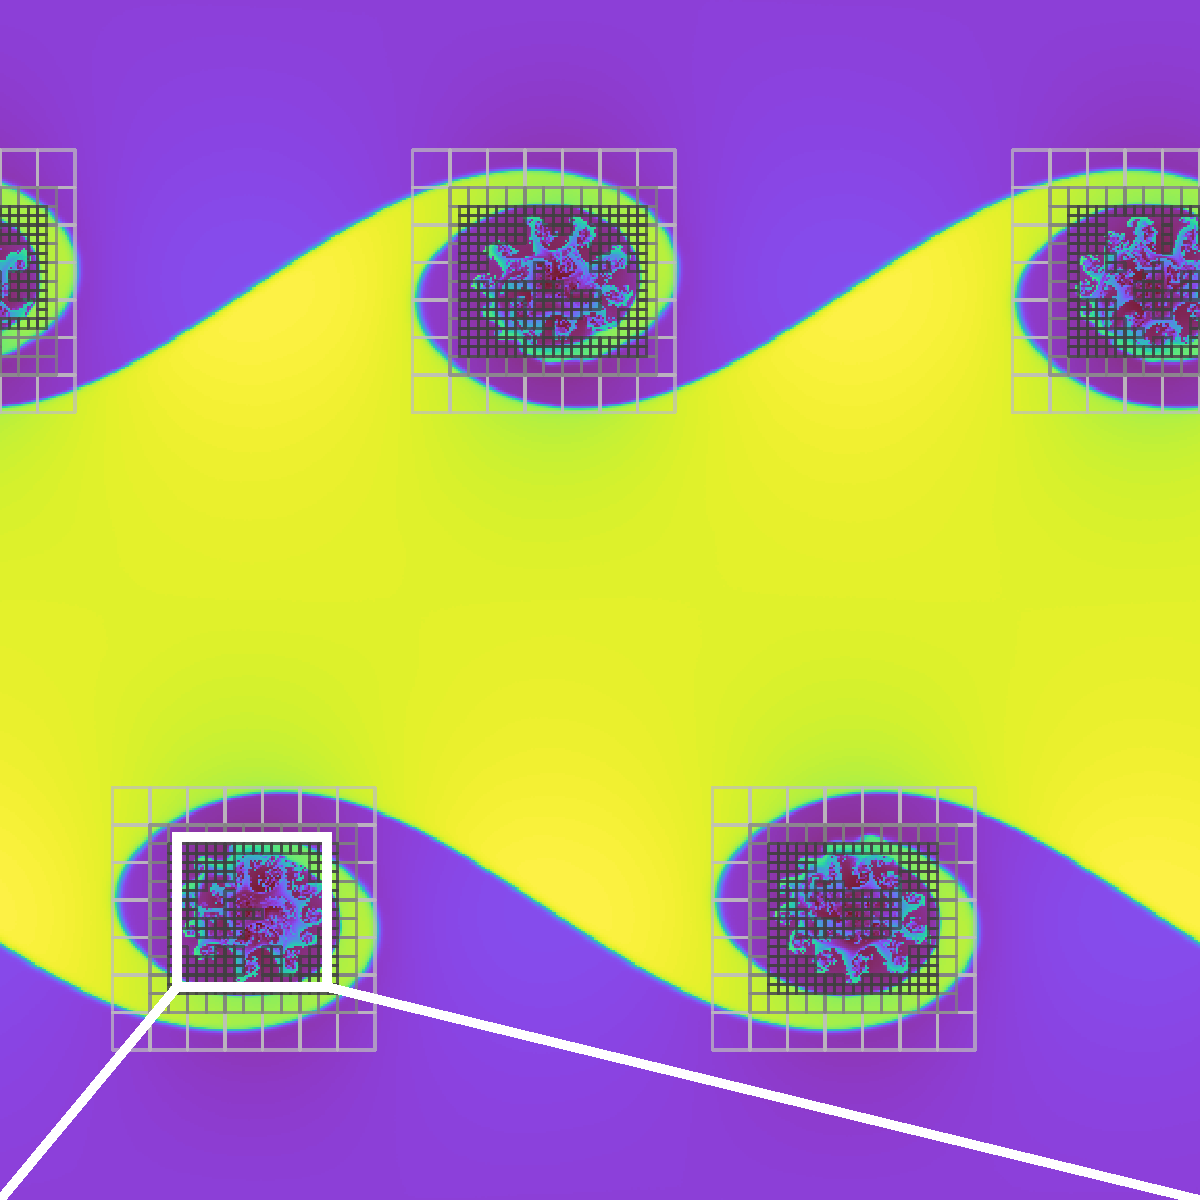
\includegraphics[width=0.9\columnwidth]{quokka_full.pdf}
    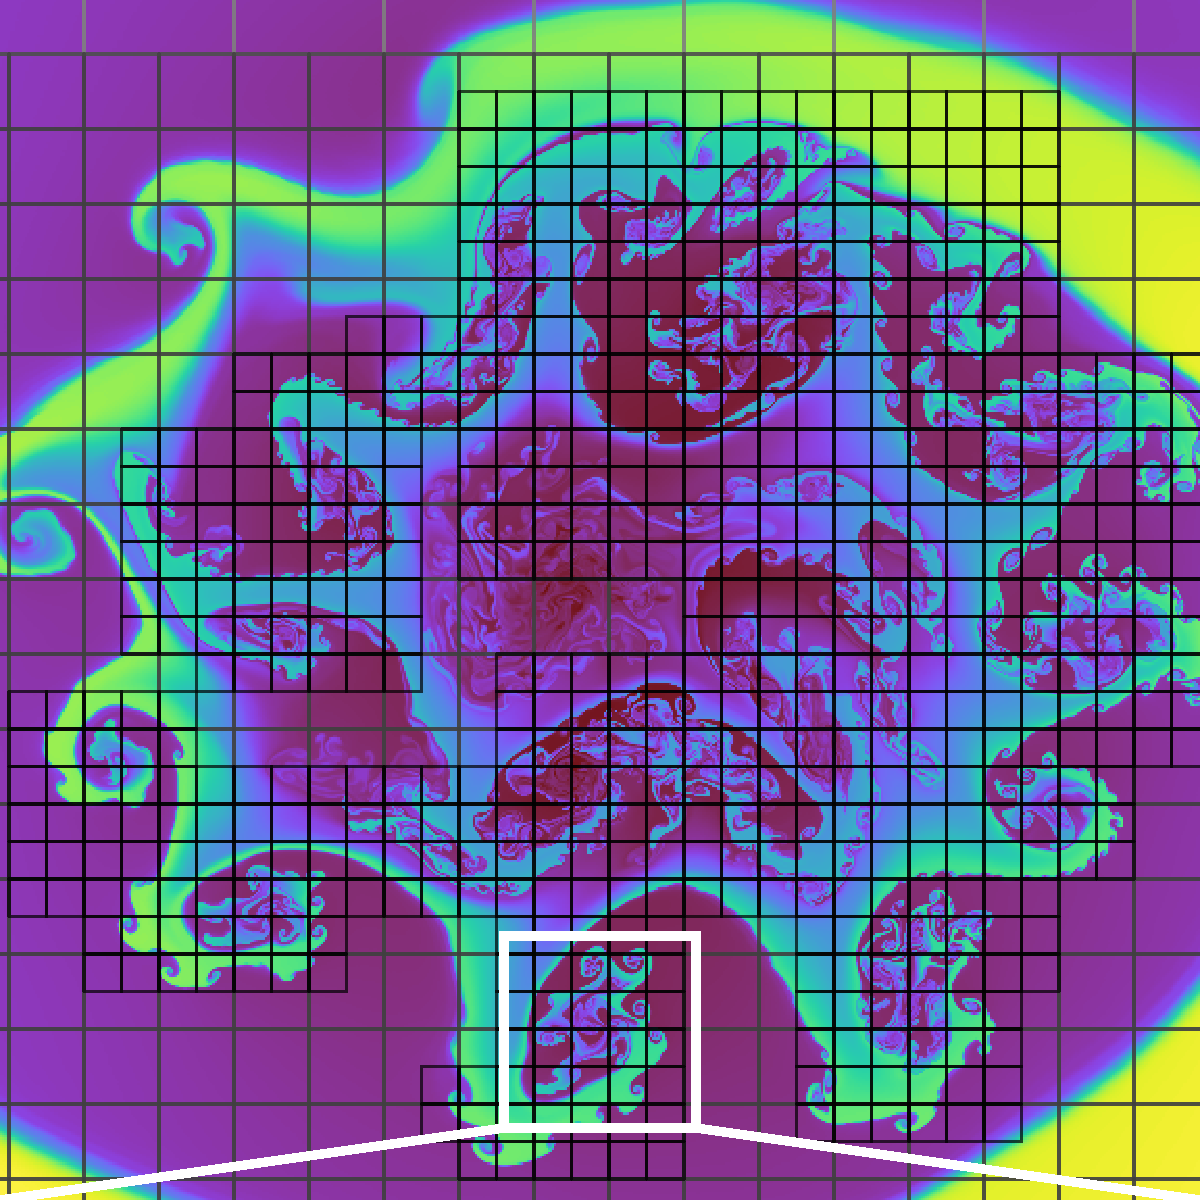
\includegraphics[width=0.9\columnwidth]{quokka_zoom.pdf}
    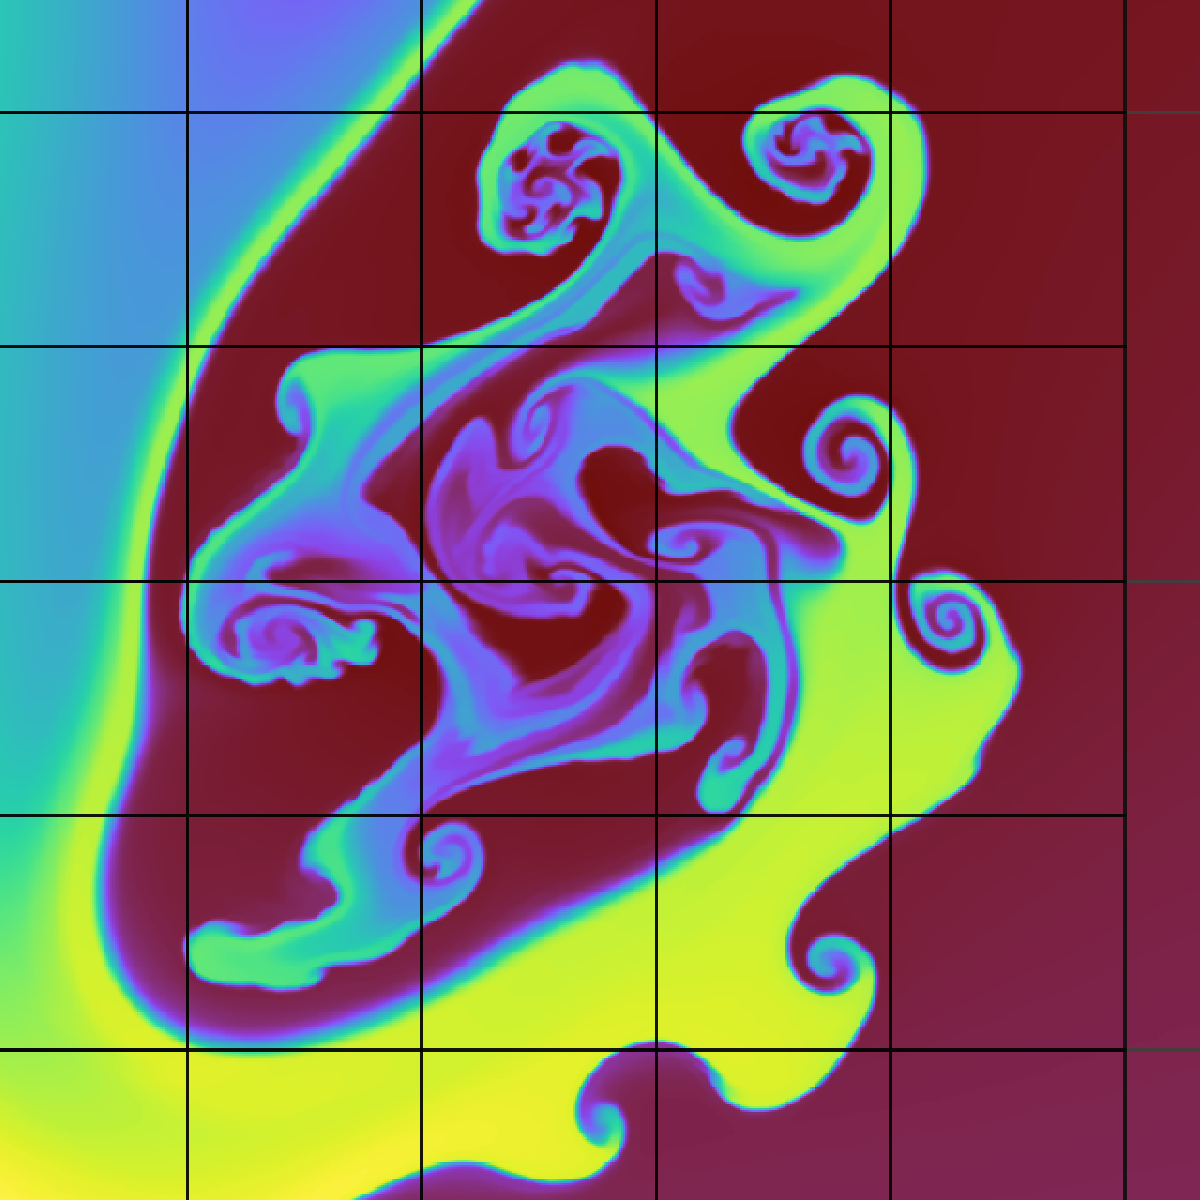
\includegraphics[width=0.9\columnwidth]{quokka_zoom2.pdf}
    \caption[]{A Kelvin-Helmholz problem with 4 levels of refinement.}
\end{figure}
\subsubsection{2D Implosion problem}

\subsection{Radiation}
\subsubsection{Marshak wave}
\subsubsection{Su-Olson problem}
\subsubsection{Radiation pressure tube}
\subsubsection{Radiation-matter energy exchange}
\subsubsection{Shadow test}
\subsubsection{Beam test}
\subsubsection{Optically-thin wind}
\subsubsection{Crooked-pipe problem}

\subsection{Radiation hydrodynamics}
\subsubsection{Subcritical radiative shock}
\subsubsection{Radiation-driven dust shell}

\section{Performance and scaling}
\label{section:performance}

\section{Discussion and Conclusions}
\label{section:discussion}
\subsection{Range of applicability}
\subsection{Planned applications}

The future is bright for radiation hydrodynamics on GPUs\dots

\section*{Acknowledgements}

This research was supported by the Australian Research Council through its Discovery Projects and Future Fellowship Funding Schemes, awards DP190101258 and FT180100375. This research was undertaken with the assistance of resources and services from the National Computational Infrastructure (NCI), which is supported by the Australian Government.

\emph{Software:} AMReX \citep{the_amrex_development_team_2021_5363443},
matplotlib \citep{Hunter:2007},
numpy \citep{harris2020array}.

%%%%%%%%%%%%%%%%%%%%%%%%%%%%%%%%%%%%%%%%%%%%%%%%%%
\section*{Data Availability}
The source code and entire commit history for \textsc{Quokka} is hosted in this public \faGithub\href{https://github.com/BenWibking/quokka-code}{GitHub repository}. The version of the source code used to produce the results in this paper as well as the output files at the final timestep for the simulations shown in the Figures are permanently archived at Zenodo DOI:XXX.

%%%%%%%%%%%%%%%%%%%% REFERENCES %%%%%%%%%%%%%%%%%%

% The best way to enter references is to use BibTeX:

\bibliographystyle{mnras}
\bibliography{quokka} % if your bibtex file is called example.bib

%%%%%%%%%%%%%%%%%%%%%%%%%%%%%%%%%%%%%%%%%%%%%%%%%%

%%%%%%%%%%%%%%%%% APPENDICES %%%%%%%%%%%%%%%%%%%%%

\appendix
\section{Asymptotic diffusion correction}
\label{appendix:asymptotic_correction}

%%%%%%%%%%%%%%%%%%%%%%%%%%%%%%%%%%%%%%%%%%%%%%%%%%


% Don't change these lines
\bsp	% typesetting comment
\label{lastpage}
\end{document}

% End of mnras_template.tex
